\subsection{LLVM}
\label{sec:llvm}
LLVM, which at one time stood for Low-Level Virtual Machine, is a popular set of open-source, modular compiler and toolchain components \cite{lattner2004llvm}.
The compiler framework was originally designed to provide analysis and transformation for an application throughout its entire lifetime: from initial compilation and linking, through to runtime and even while the application was offline (see Figure \ref{fig:llvmarch}).
\begin{figure*}
    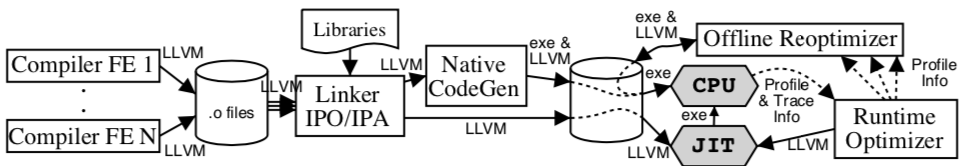
\includegraphics[width=\textwidth]{images/llvm-architecture.png}
    \caption{ The LLVM Compiler Framework Architecture \cite{lattner2004llvm}.}
    \label{fig:llvmarch}
    \Description[]{}
\end{figure*}
To achieve this ambitious goal, the framework utilizes a well defined, human-readable, intermediate representation (IR) called LLVM IR.
The IR, which is initially generated by the front end, can be packaged with the target architecture binary that includes profiling instructions for later runtime compilation (JIT) as well as more aggressive offline optimizations.
Several important characteristics of LLVM IR are as follows:
\begin{itemize}
    \item The IR maintains Static Single Assignment (SSA) form with unlimited virtual registers.
    \item Each register is of one of four primitive types: boolean, integer, floating-point or pointer.
    \item Similar to RISC, memory operations are carried out in registers, while operations between registers and memory use Load and Store instructions.
    \item The IR is limited to 31 opcodes.
    \item The IR is organized into basic blocks which must be composed into valid control flow graphs, simplifying the work required for various optimizations. 
\end{itemize}

\begin{lstlisting}[float,floatplacement=H,
caption={LLVM IR for a function returning x * y + z \cite{LLVM_Jit_Tutorial}.},
label=lst:llvm_ir]
define i32 @mul_add(i32 %x, i32 %y, i32 %z) {
    entry:
    %tmp = mul i32 %x, %y
    %tmp2 = add i32 %tmp, %z
    ret i32 %tmp2
}\end{lstlisting}

This report will focus on LLVM's JIT component, which can be accessed through the MCJIT application programming interface (API).
The MCJIT framework provides an API that accepts IR, generates optimized machine code, and provides a function pointer for calling the generated code.
The JIT compiler offers several levels of optimization: none, less, default, and aggressive.
It should be noted that the JIT compiler by default does not perform any IR optimizations or transformations.
Instead, a developer must pass the generated IR to a PassManager with specific optimizations they intend to apply.
These passes can be categorized as analysis passes, or transformation passes \cite{LLVM_Passes}:
\begin{itemize}
    \item Analysis Passes: collects information about IR for use later by transformations, for debugging or for visualization. 
    A few examples are \textit{print-callgraph}, \textit{print-function}, and \textit{iv-users} for printing the users of a particular induction variable. There are roughly 40 such passes available.
    \item Transformation Passes: These typically modify IR. Examples include \textit{adce} for dead code elimination, \textit{instcombine} for combining redundant instructions, or peephole optimizing, and \textit{tailcallelim} for eliminating tail calls. There are roughly 60 such passes available.
\end{itemize}
Generated IR can then be used by the ExecutionEngine to generate code for the target architecture.
Before a function is executed by the ExecutionEngine, it first checks if the code cache, or ObjectCache, contains a copy.
If the function could not be found, the compiler will generate the JIT code and store it in the ObjectCache before execution \cite{LLVM_MCJIT}.
It is worth noting that a newer JIT API, called ORCJIT, is also part of the LLVM project.
ORCJIT, or On-Request-Compilation JIT, is intended to complement the MCJIT API -- which compiles eagerly, by adding support for both lazy and concurrent compilations \cite{LLVM_ORCJIT}.